\thispagestyle{foliage-header}
\poemtitle{O Christmas Tree}
\begin{multicols}{2}
\begin{verse}
O Christmas Tree, O Christmas tree,\\
How lovely are your branches!\\
O Christmas Tree, O Christmas tree,\\
How lovely are your branches!\\
Not only green in summer’s heat,\\
But also winter’s snow and sleet.\\
O Christmas tree, O Christmas tree,\\
How lovely are your branches!\\!
\vfill*{}

O Christmas Tree, O Christmas tree,\\*
Of all the trees most lovely;\\*
O Christmas Tree, O Christmas tree,\\*
Of all the trees most lovely.\\*
Each year you bring to us delight\\*
With brightly shining Christmas light!\\*
O Christmas Tree, O Christmas tree,\\*
Of all the trees most lovely.\\!

O Christmas Tree, O Christmas tree,\\
We learn from all your beauty;\\
0 Christmas Tree, O Christmas tree,\\
We learn from all your beauty.\\
Your bright green leaves with festive cheer,\\
Give hope and strength throughout the year.\\
O Christmas Tree, O Christmas tree,\\
We learn from all your beauty.\\!
\end{verse}
\end{multicols}
\begin{tikzpicture}[remember picture,overlay]
\draw  let \p1=($(current page.south)-(current page footer area.north)$),
\n1={veclen(\x1,\y1)} in
node [inner sep=0,outer sep=0,above right] 
at ([xshift=-2.5cm]current page.south west){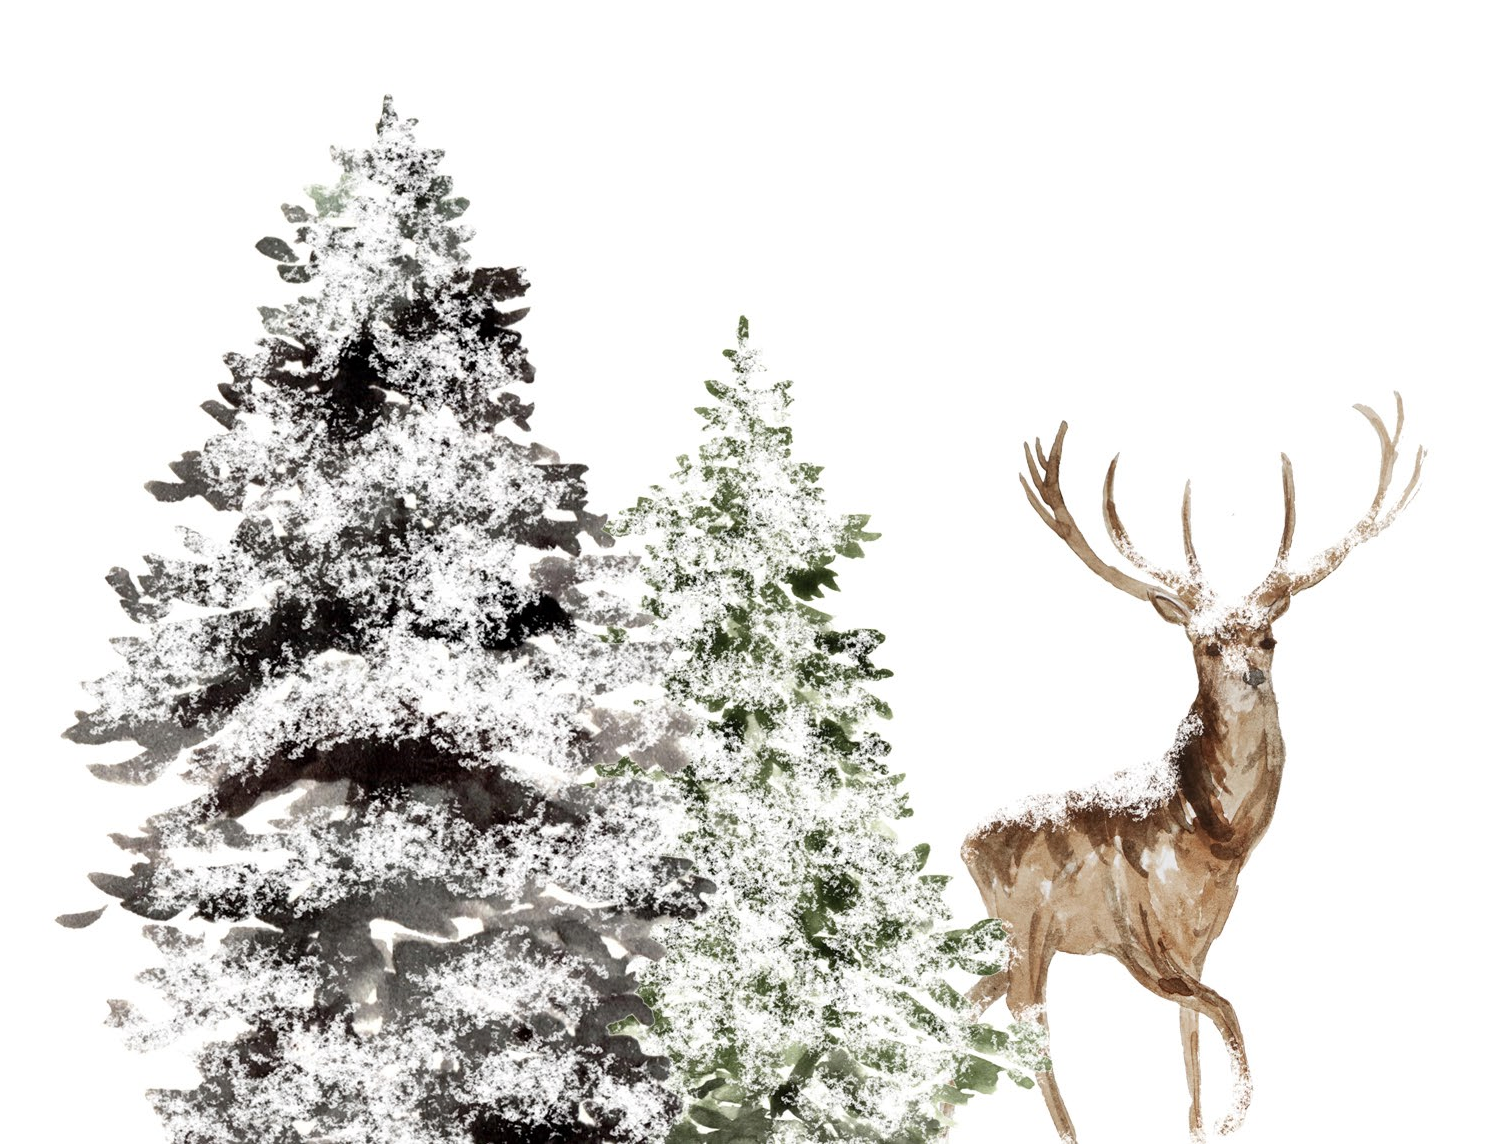
\includegraphics[width=0.7\paperwidth]{images/deer-2}};
\end{tikzpicture}
\pagebreak
